
\documentclass{acm_proc_article-sp}
\usepackage{hyperref}

\begin{document}

\title{Linked Data-driven Web Components}
\subtitle{}

\numberofauthors{1} %  in this sample file, there are a *total*
\author{
% 1st. author
\alignauthor
Ali Khalili\\
       \affaddr{Dept. of Computer Science}\\
       \affaddr{VU University Amsterdam}\\
       \affaddr{The Netherlands}\\
       \email{a.khalili@vu.nl}
}


\maketitle
\begin{abstract}
This paper provides a ...

\end{abstract}


\section{Introduction}
The


The remainder of this article...

\section{Related Work}

Web Components and the Semantic Web~\cite{pahl2011}

\section{Web Components}
\emph{Web Components} are a set of W3C standards that enable the creation of reusable widgets or components in Web documents and Web applications.
Web components aim to bring \emph{Component-Based Software Development} (CBSD) to the World Wide Web.
Some advantages of CBSD approach are reusibility, replacability, extensibility, encapsulation and independence.

\section{Linked Data-driven Web Components}

Definition

We define a \emph{Linked Data-driven} (LD-R) Web Component as a Web component which employs RDF data model for representing its content and specification (i.e. metadata about the component).

\subsection{Features}

Linked Data-driven Web components provide the following features:

\begin{itemize}

\item \emph{Fine-grained Web applications}.
Resource Description Framework (RDF) provides a common data model that allows data-driven components to be created, shared and integrated in a structured way across different applications. \autoref{fig:architecture} depicts the 5 main component levels in a Linked Data-driven Web application.
The dataflow in the application starts from the \emph{Dataset} component which handles all the events related to a set of resources embedded in a named graph.
The next level is the \emph{Resource} component which is identified by a URI and indicates what is described in the application.
A resource is specified by a set of properties which are handled by the \emph{Property} component. Properties can be either individual or aggregate when combining multiple features of a resource.
Each property is instantiated by a value (or mutiple values in case of an aggreagte object). 
The values of properties are controled by the \emph{Object} component which invokes different components to view, edit and browse the property values.
\emph{Viewer}, \emph{Editor} and \emph{Browser} components are terminals in the LD-R single directional data flow where customized user-generated components can be plugged into the system.

\begin{figure}[tb]
  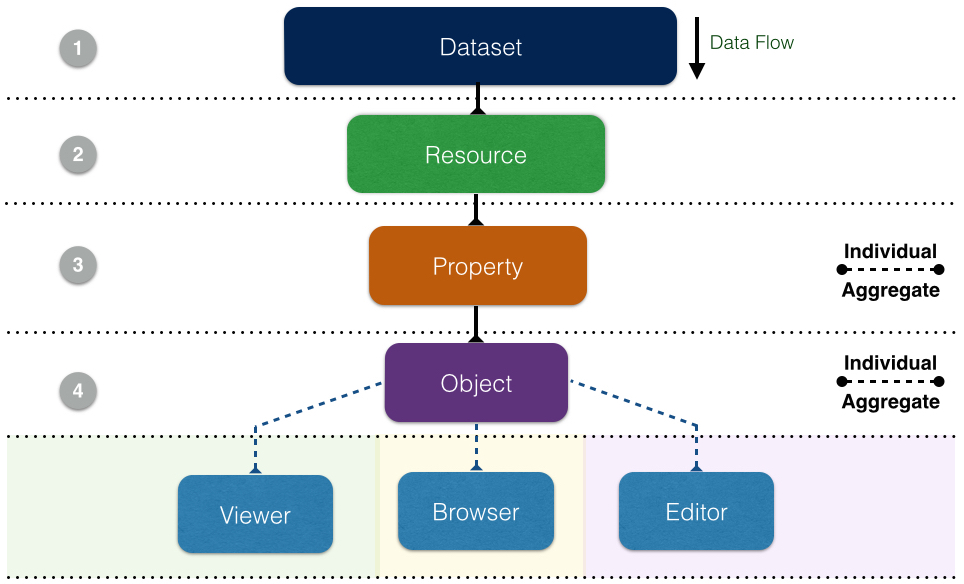
\includegraphics[width=.9\linewidth]{images/architecture.jpg}
  \caption{Architecture of LD-R Applications.}
  \label{fig:architecture}
\end{figure}

In addition to the fine-grained component architecture, LD-R Web applications provide a fine-grained access control over the data provided by the components.
RDF-based access control in LD-R applications operates at four different granularities provided by Dataset, Resource, Property and Object component levels.
For example, we can restrict access to a specific property of a specific resource in a certain dataset.

\begin{figure}[tb]
  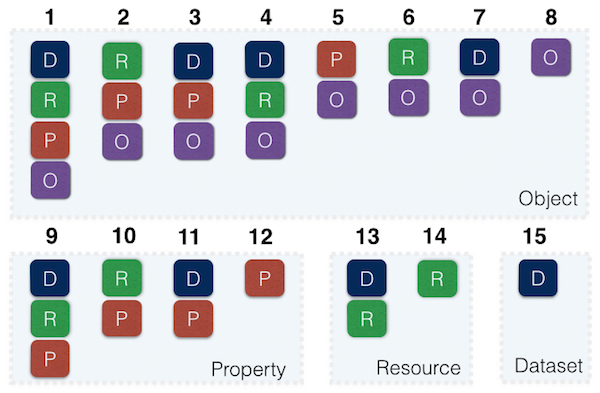
\includegraphics[width=.9\linewidth]{images/scopes.jpg}
  \caption{LD-R Scopes.}
  \label{fig:scopes}
\end{figure}

\item \emph{Customization and Personalization}.
LD-R provide a versatile approach for context adaptation.
A context can be a specific domain of interest, a specific user requirments or both.
In order to enable customization and personalization, LD-R exploits the concept of \emph{Scope}.
A scope is defiened as a directed combination of Dataset, Resource, Property and Object components (cf. \autoref{fig:scopes}).
Each scope conveys a certain level of specificity on a given context ranging from 1 (most specific) to 15 (least specfic).


- scopes and user-scopes

\item \emph{Component/Content Visibility and Reusability}.

- RDFa, Microdata



\end{itemize}



\subsection{Life Cycle}

\begin{figure}[tb]
  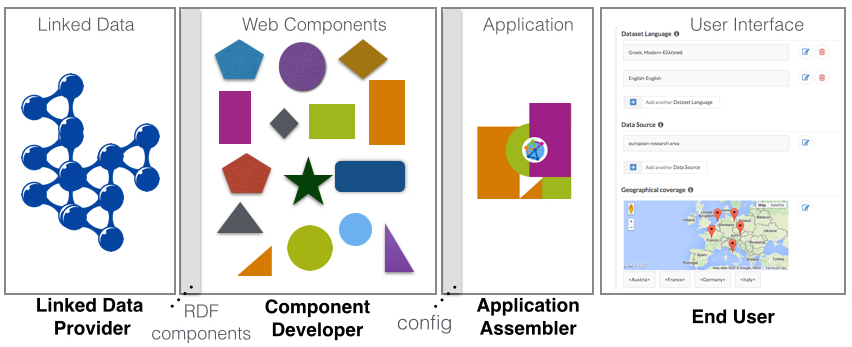
\includegraphics[width=1\linewidth]{images/lifecycle.jpg}
  \caption{Life-cycle}
\end{figure}

\section{Implementation}

http://ld-r.org


\begin{figure}[tb]
  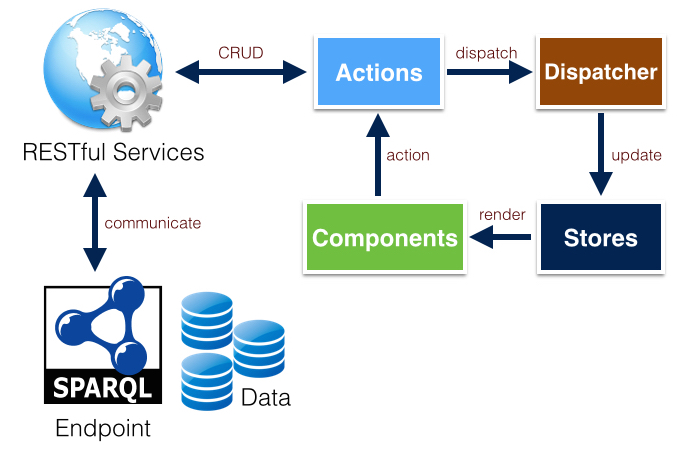
\includegraphics[width=.9\linewidth]{images/dataflow.jpg}
  \caption{Data Flow}
\end{figure}

\begin{figure}[tb]
  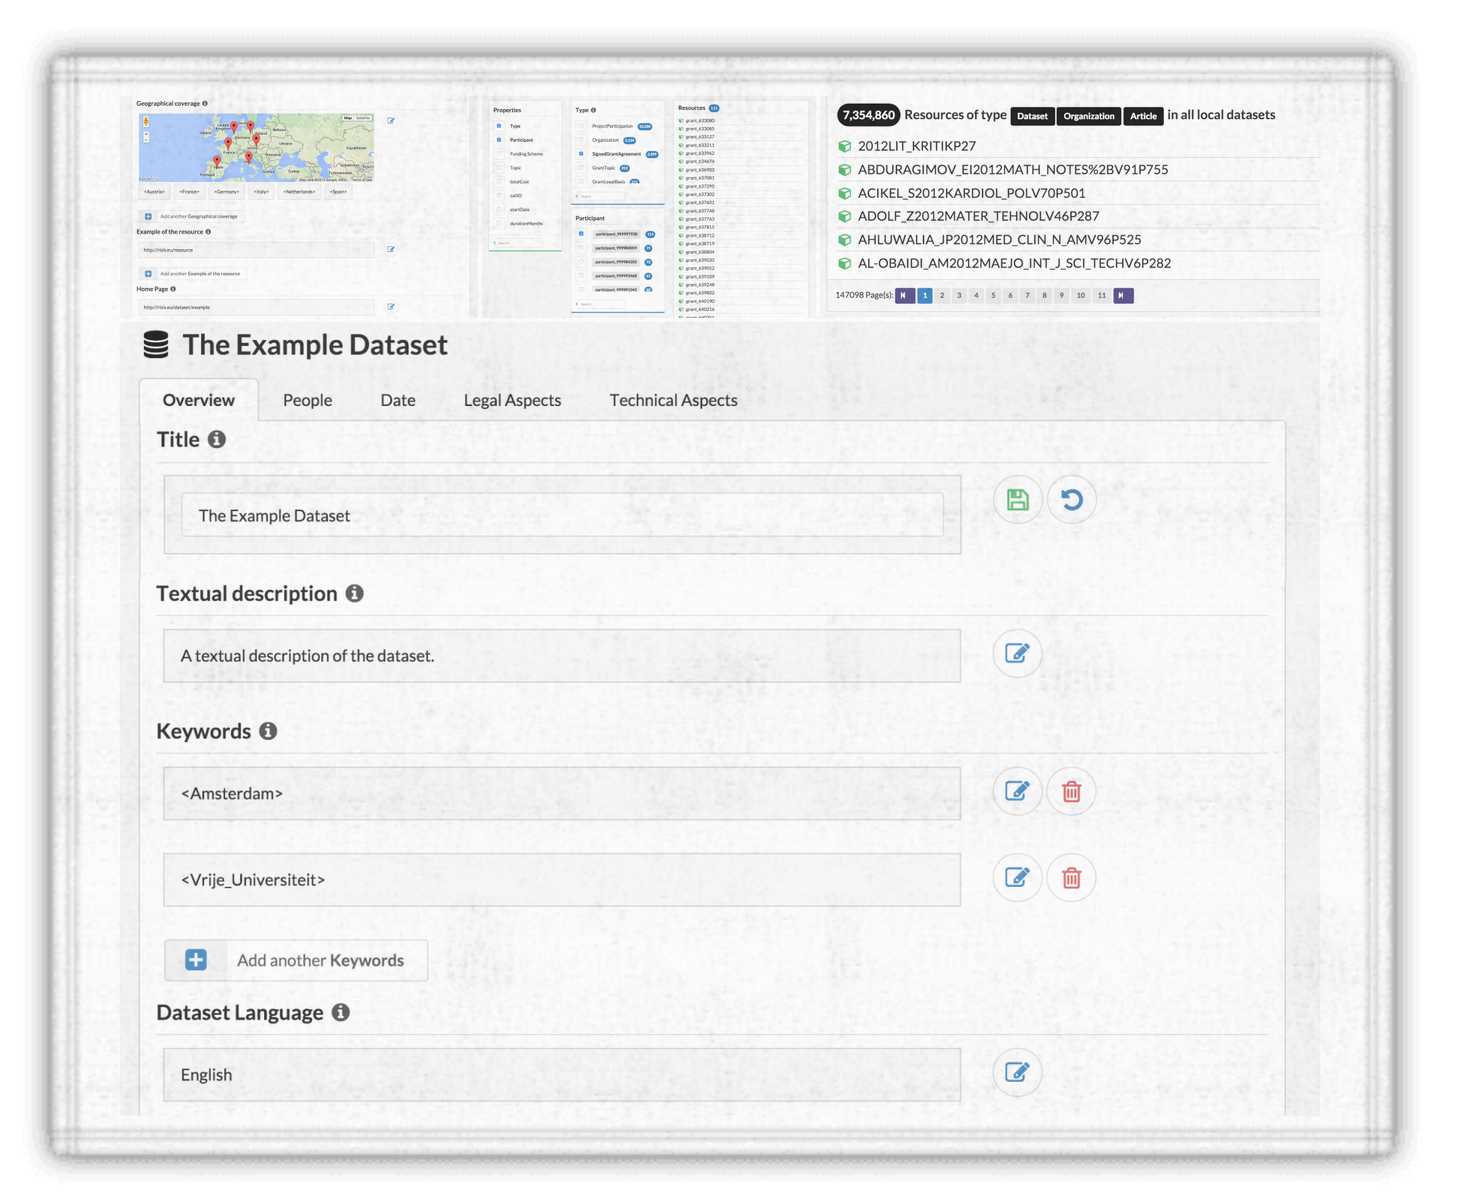
\includegraphics[width=.9\linewidth]{images/screenshot.png}
  \caption{Screenshot}
\end{figure}

\section{Evaluation}

RISIS

OpenPhacts

\section{Conclusion and Future Work}

\section{Aknowledgement}
We would like to thank our colleagues from the KRR research group at VU University Amsterdam for their helpful comments during the development of the LD-R framework. This work was supported by a grant from the European Union’s 7th Framework Programme provided for the project RISIS (GA no. 313082).


\bibliographystyle{abbrv}
\bibliography{refs}

\end{document}
